\documentclass[11pt]{standalone}
\usepackage{amssymb}
\usepackage{amsmath}
\usepackage[no-math]{fontspec}
\usepackage{unicode-math}
\usepackage{libertinus}
\usepackage{pgf,xcolor}
\usepackage{tikz}
\usetikzlibrary{arrows.meta, backgrounds}
\usepackage{pgfplots}
\pgfplotsset{compat=newest}
\usepgfplotslibrary{groupplots}

\definecolor{my_darkgray}{HTML}{484949}
\definecolor{my_lightgray}{HTML}{F3F4F4}
\definecolor{my_darkblue}{HTML}{005A94}
\definecolor{my_lightblue}{HTML}{CCDEE9}
\definecolor{my_yellow}{HTML}{FFEC7F}
\definecolor{my_red}{HTML}{E60000}
\definecolor{my_orange}{HTML}{E87846}

\begin{document}
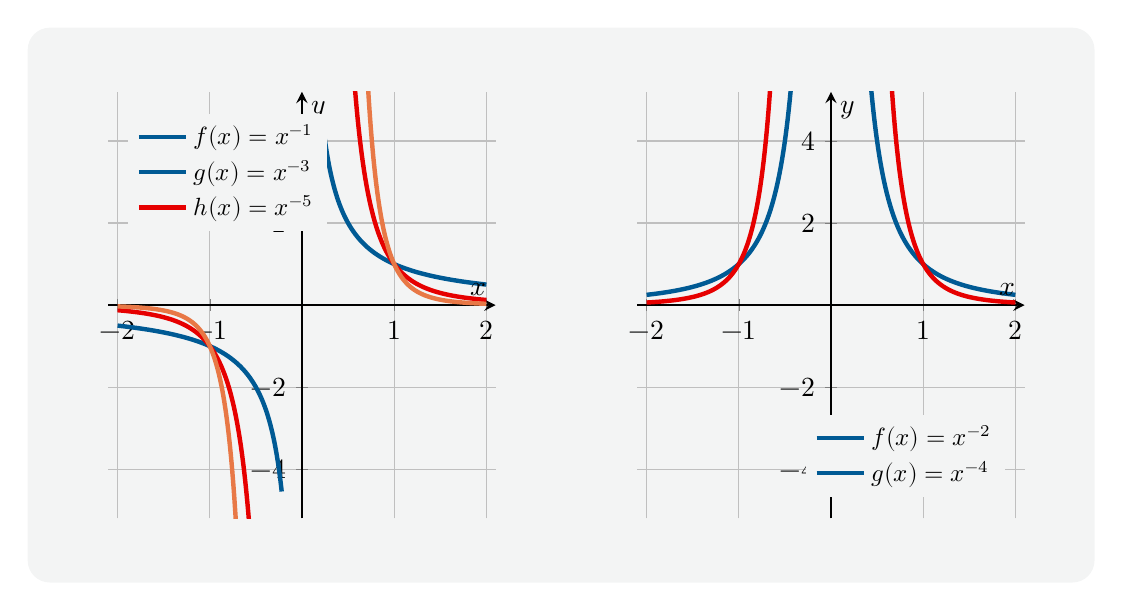
\begin{tikzpicture}[
    show background rectangle,
    background rectangle/.style={fill=my_lightgray, rounded corners=8pt},
    inner frame sep=0.8cm
]
\begin{groupplot}[
    group style={
        group size=2 by 1,
        horizontal sep=1.8cm,
    },
    % Shared axis style
    axis lines=center,
    xlabel={$x$},
    ylabel={$y$},
    height=7cm, width=6.5cm,
    xmin=-2.1, xmax=2.1,
    ymin=-5.2, ymax=5.2,
    xtick={-2,-1,0,1,2},
    ytick={-4,-2,0,2,4},
    grid=both,
    axis line style={thick},
    % Clip curves that escape the y-range near the pole at x=0
    restrict y to domain=-5.5:5.5,
    legend style={
        font=\small,
        at={(0.05, 0.95)},
        anchor=north west,
        draw=none,
        fill=my_lightgray,
    },
    legend cell align=left,
]

% Left panel: odd negative exponents — point-symmetric about the origin.
% Each function is split into a left branch (x < 0) and a right branch (x > 0).
% The split point is chosen conservatively so the curve exits the y-range
% well before reaching x = 0.
\nextgroupplot
% f(x) = x^{-1} = 1/x
\addplot[draw=my_darkblue, samples=300, ultra thick, domain=-2:-0.22]{x^(-1)};
\addplot[draw=my_darkblue, samples=300, ultra thick, domain= 0.22:2] {x^(-1)};
\addlegendentry{$f(x)=x^{-1}$}
% g(x) = x^{-3} = 1/x^3
\addplot[draw=my_red, samples=300, ultra thick, domain=-2:-0.55]{x^(-3)};
\addplot[draw=my_red, samples=300, ultra thick, domain= 0.55:2] {x^(-3)};
\addlegendentry{$g(x)=x^{-3}$}
% h(x) = x^{-5} = 1/x^5
\addplot[draw=my_orange, samples=300, ultra thick, domain=-2:-0.68]{x^(-5)};
\addplot[draw=my_orange, samples=300, ultra thick, domain= 0.68:2] {x^(-5)};
\addlegendentry{$h(x)=x^{-5}$}

% Right panel: even negative exponents — symmetric about the y-axis.
% Both branches are always positive; legend sits in the lower-right corner.
\nextgroupplot[
    legend style={
        font=\small,
        at={(0.95, 0.05)},
        anchor=south east,
        draw=none,
        fill=my_lightgray,
    },
]
% f(x) = x^{-2} = 1/x^2
\addplot[draw=my_darkblue, samples=300, ultra thick, domain=-2:-0.22]{x^(-2)};
\addplot[draw=my_darkblue, samples=300, ultra thick, domain= 0.22:2] {x^(-2)};
\addlegendentry{$f(x)=x^{-2}$}
% g(x) = x^{-4} = 1/x^4
\addplot[draw=my_red, samples=300, ultra thick, domain=-2:-0.55]{x^(-4)};
\addplot[draw=my_red, samples=300, ultra thick, domain= 0.55:2] {x^(-4)};
\addlegendentry{$g(x)=x^{-4}$}

\end{groupplot}
\end{tikzpicture}
\end{document}
